\documentclass[aspectratio=169]{beamer}
\usetheme{Madrid}
\usecolortheme{default}
\usepackage[utf8]{inputenc}
\usepackage[T5]{fontenc}
\usepackage{graphicx}
\usepackage{hyperref}
\usepackage{booktabs}
\usepackage{tikz}

\setbeamertemplate{caption}[numbered]
\renewcommand{\figurename}{Hình}

\title[Buổi 1: AI \& Nghề Kế toán]{Trí tuệ Nhân tạo cho Kế toán \\ \vspace{0.3cm} \Large Buổi 1: Tổng quan Ứng dụng AI trong Kế toán}
\author{Đại học Đông Á}
\date{\today}

\begin{document}

% SLIDE 1
\begin{frame}
    \titlepage
\end{frame}

% SLIDE 2
\begin{frame}{Nội dung Chương trình Buổi học}
    \tableofcontents
\end{frame}

% SLIDE 3
\begin{frame}{Năng lực đạt được sau buổi học}
    \begin{itemize}
        \item \textbf{Về Lý thuyết (LT):} Nắm vững nền tảng Hệ thống Thông tin Kế toán (AIS); Phân biệt rõ sự khác nhau giữa AI, Machine Learning và Deep Learning trong bối cảnh kế toán tài chính.
        \item \textbf{Về Thực hành (TH):} Có khả năng sử dụng các Generative AI (ChatGPT, Copilot, Gemini) để đóng vai (Role-play) hỗ trợ giải đáp các chuẩn mực kế toán cơ bản.
        \item \textbf{Về Tư duy nghề nghiệp:} Chấp nhận và thích nghi với sự thay đổi của nghề kế toán trong kỷ nguyên AI; Nhận thức AI là công cụ hỗ trợ (Copilot), không phải mối đe dọa thay thế hoàn toàn kế toán viên.
    \end{itemize}
\end{frame}

\section{1. Nền tảng Hệ thống Thông tin Kế toán (AIS)}

% SLIDE 4
\begin{frame}{Mở đầu - Câu chuyện kinh doanh (Case Study: S\&S)}
    \begin{itemize}
        \item \textbf{Bối cảnh:} Mở doanh nghiệp S\&S chuyên bán lẻ.
        \item \textbf{Các quyết định cần đưa ra:} 
        \begin{itemize}
            \item Định giá sản phẩm như thế nào?
            \item Quản lý dòng tiền ra sao?
            \item Quy trình thuê nhân viên và tính lương?
        \end{itemize}
        \item \textbf{Giải pháp:} Tất cả đều phụ thuộc vào một \textbf{Hệ thống thông tin} để đưa ra quyết định chính xác.
    \end{itemize}
\end{frame}

% SLIDE 5
\begin{frame}{Hệ thống (System) là gì?}
    \begin{itemize}
        \item \textbf{Định nghĩa:} Tập hợp các phương pháp, quy trình để thực hiện một mục tiêu.
        \item \textbf{Hệ thống con (Subsystem):} Một hệ thống lớn (Đại học) bao gồm nhiều hệ thống con (Khoa Kế toán, Khoa CNTT).
        \item \textbf{Mục tiêu đồng nhất (Goal congruence):} Khi hệ thống con đóng góp vào mục tiêu chung.
        \item \textbf{Xung đột mục tiêu (Goal conflict):} Khi lợi ích hệ thống con đi ngược với hệ thống lớn.
    \end{itemize}
\end{frame}

% SLIDE 6
\begin{frame}{Dữ liệu (Data) vs. Thông tin (Information)}
    \begin{columns}
        \column{0.5\textwidth}
        \textbf{Dữ liệu (Data):}
        \begin{itemize}
            \item Các sự kiện thô được thu thập, ghi chép.
            \item Ví dụ: Số tiền, ngày tháng, tên khách hàng.
        \end{itemize}
        
        \column{0.5\textwidth}
        \textbf{Thông tin (Information):}
        \begin{itemize}
            \item Dữ liệu đã được tổ chức, xử lý.
            \item Mang lại ý nghĩa cho người ra quyết định.
            \item Ví dụ: Báo cáo doanh thu tháng.
        \end{itemize}
    \end{columns}
    \vspace{0.5cm}
    \begin{center}
        \textit{Lưu ý: Nguy cơ "Quá tải thông tin" (Information Overload) khi xử lý quá nhiều dữ liệu.}
    \end{center}
\end{frame}

% SLIDE 7
\begin{frame}{7 Đặc tính của Thông tin hữu ích (Phần 1)}
    \begin{enumerate}
        \item \textbf{Phù hợp (Relevant):} Hỗ trợ dự báo hoặc xác nhận kết quả trong quá khứ. Giảm sự không chắc chắn.
        \item \textbf{Đáng tin cậy (Reliable):} Chính xác, không thiên vị (bias) và đại diện trung thực cho các sự kiện kinh tế.
        \item \textbf{Đầy đủ (Complete):} Không bỏ sót bất kỳ khía cạnh quan trọng nào của sự kiện.
        \item \textbf{Kịp thời (Timely):} Có sẵn ngay lúc cần thiết để ra quyết định.
    \end{enumerate}
\end{frame}

% SLIDE 8
\begin{frame}{7 Đặc tính của Thông tin hữu ích (Phần 2)}
    \begin{enumerate}
        \setcounter{enumi}{4}
        \item \textbf{Dễ hiểu (Understandable):} Trình bày rõ ràng, định dạng dễ đọc cho người dùng cuối (Ban giám đốc).
        \item \textbf{Có thể xác minh (Verifiable):} Hai người hoặc hệ thống độc lập cùng ra một kết quả tương tự từ cùng nguồn dữ liệu.
        \item \textbf{Dễ tiếp cận (Accessible):} Có sẵn ở định dạng dễ sử dụng và tại thời điểm người dùng cần.
    \end{enumerate}
\end{frame}

% SLIDE 9
\begin{frame}{Giá trị của Thông tin (Value of Information)}
    \begin{itemize}
        \item \textbf{Định nghĩa:} Giá trị của Thông tin = Lợi ích của thông tin trừ đi Chi phí tạo ra nó.
        \item \textbf{Lợi ích:} 
        \begin{itemize}
            \item Giảm rủi ro kinh doanh.
            \item Cải thiện quyết định chiến lược.
            \item Tăng hiệu suất hoạt động.
        \end{itemize}
        \item \textbf{Chi phí:} Thời gian, công sức thu thập, xử lý và lưu trữ.
        \item \textbf{Sự can thiệp của AI:} Làm giảm triệt để chi phí tạo ra thông tin (tự động hóa).
    \end{itemize}
\end{frame}

% SLIDE 10
\begin{frame}{Hệ thống Thông tin Kế toán (AIS) là gì?}
    AIS là hệ thống thu thập, ghi chép, lưu trữ và xử lý dữ liệu kế toán để tạo ra thông tin. \\ \vspace{0.3cm}
    \textbf{6 Thành phần của một AIS:}
    \begin{enumerate}
        \item \textbf{Con người (People):} Người vận hành hệ thống.
        \item \textbf{Thủ tục (Procedures):} Các quy tắc thủ công hoặc tự động.
        \item \textbf{Dữ liệu (Data):} Dữ liệu về tổ chức và hoạt động kinh doanh.
        \item \textbf{Phần mềm (Software):} Ứng dụng xử lý dữ liệu.
        \item \textbf{Hạ tầng CNTT (IT Infrastructure):} Máy tính, máy chủ, mạng lưới.
        \item \textbf{Kiểm soát nội bộ (Internal Controls):} Bảo mật và an toàn dữ liệu.
    \end{enumerate}
\end{frame}

\section{2. Sự tiến hóa của Nghề Kế toán \& Trí tuệ Nhân tạo}

% SLIDE 11
\begin{frame}{Sự chuyển dịch vai trò của Kế toán viên}
    \begin{itemize}
        \item \textbf{Kỷ nguyên Giấy bút (Bookkeeper):} Tập trung vào việc ghi chép lịch sử giao dịch một cách máy móc.
        \item \textbf{Kỷ nguyên Dữ liệu (Data Analyst):} Sử dụng dữ liệu phần mềm ERP để phân tích và tham mưu.
        \item \textbf{Kỷ nguyên AI (Strategic Advisor):} Trở thành cố vấn chiến lược, sử dụng mô hình dự báo tương lai thay vì chỉ báo cáo quá khứ.
    \end{itemize}
\end{frame}

% SLIDE 12
\begin{frame}{Sức ép thay đổi - "Thiên nga đen" (Black Swan)}
    \begin{columns}
        \column{0.6\textwidth}
        \begin{itemize}
            \item \textbf{Thiên nga đen:} Khái niệm chỉ những sự kiện cực kỳ khó lường, gây chấn động mạnh và để lại hậu quả to lớn (Ví dụ: Đại dịch Covid-19, khủng hoảng tài chính toàn cầu).
            \item \textbf{Thách thức của Kế toán truyền thống:} Các mô hình báo cáo tĩnh và quy tắc cứng nhắc sụp đổ khi đối mặt với biến động bất ngờ.
            \item \textbf{Giải pháp:} Cần hệ thống thông tin linh hoạt (AI) để dự báo và phản ứng kịp thời.
        \end{itemize}
        \column{0.4\textwidth}
        \centering
        % 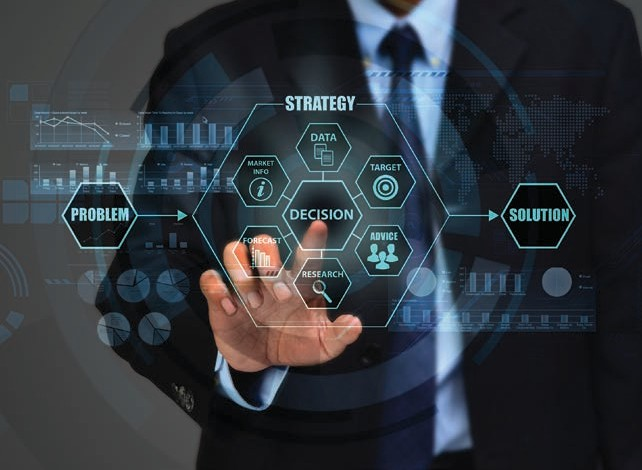
\includegraphics[width=\textwidth]{images/Day_01/img_1.jpeg}
        \textit{(Hình ảnh Thiên nga đen)}
    \end{columns}
\end{frame}

% SLIDE 13
\begin{frame}{Lịch sử và Định nghĩa về Trí tuệ Nhân tạo (AI)}
    \begin{itemize}
        \item \textbf{Định nghĩa:} AI là khả năng của máy móc thực hiện các tác vụ đòi hỏi nhận thức và suy luận tương tự con người. Không phải phép màu, mà là khoa học máy tính + thống kê + dữ liệu khổng lồ.
        \item \textbf{Các cột mốc lịch sử:}
        \begin{itemize}
            \item \textbf{1950:} Alan Turing và "Phép thử Turing" (Turing Test).
            \item \textbf{1956:} Thuật ngữ "Artificial Intelligence" ra đời tại Hội nghị Dartmouth.
            \item \textbf{Hiện tại:} Sự bùng nổ của Generative AI và các mô hình ngôn ngữ lớn (LLMs).
        \end{itemize}
    \end{itemize}
\end{frame}

% SLIDE 14
\begin{frame}{Các "Mùa đông AI" (AI Winters)}
    \begin{itemize}
        \item \textbf{Khái niệm:} Là những giai đoạn (thập niên 70, 80) khi nghiên cứu AI bị đình trệ, mất niềm tin từ công chúng và cắt giảm nguồn vốn đầu tư.
        \item \textbf{Nguyên nhân trong quá khứ:} Phần cứng máy tính quá yếu, thiếu dữ liệu huấn luyện, thuật toán chưa giải quyết được bài toán thực tế.
        \item \textbf{Tại sao hiện nay AI bùng nổ (Không còn Mùa đông)?}
        \begin{itemize}
            \item Nguồn dữ liệu (Big Data) khổng lồ đã được số hóa.
            \item Sức mạnh điện toán đám mây (Cloud Computing).
            \item Chip xử lý đồ họa (GPU/TPU) siêu tốc.
        \end{itemize}
    \end{itemize}
\end{frame}

% SLIDE 15
\begin{frame}{Phân biệt AI, Machine Learning và Deep Learning}
    \begin{itemize}
        \item \textbf{Trí tuệ nhân tạo (AI):} Khái niệm bao trùm - Máy móc hành động như con người.
        \item \textbf{Học máy (Machine Learning - ML):} Tập con của AI. Dùng thuật toán học từ dữ liệu mà không cần lập trình rõ ràng mọi quy tắc (VD: Dự đoán doanh thu).
        \item \textbf{Học sâu (Deep Learning):} Tập con của ML. Sử dụng Mạng nơ-ron nhân tạo nhiều lớp (Neural Networks) để xử lý dữ liệu phi cấu trúc cực kỳ phức tạp (hình ảnh hóa đơn, giọng nói).
    \end{itemize}
\end{frame}

% SLIDE 16
\begin{frame}{Các loại Học máy (Machine Learning Types)}
    \begin{itemize}
        \item \textbf{Học có giám sát (Supervised Learning):} Máy học từ dữ liệu đã có nhãn. (VD: Phân loại một email là rác hay không rác dựa trên dữ liệu mẫu).
        \item \textbf{Học không giám sát (Unsupervised Learning):} Máy tự tìm ra quy luật từ tập dữ liệu không nhãn. (VD: Phân cụm khách hàng, phát hiện giao dịch gian lận bất thường).
        \item \textbf{Học tăng cường (Reinforcement Learning):} Máy học thông qua quá trình thử/sai và nhận phần thưởng/hình phạt.
    \end{itemize}
\end{frame}

% SLIDE 17
\begin{frame}{Trí tuệ Con người vs. Trí tuệ Nhân tạo}
    \begin{table}
        \centering
        \small
        \begin{tabular}{p{4.2cm}p{4.8cm}p{4.8cm}}
            \toprule
            \textbf{Tiêu chí} & \textbf{AI} & \textbf{Con người} \\
            \midrule
            \textbf{Tác vụ lặp lại quy mô lớn} & Xử lý hàng triệu dòng dữ liệu siêu tốc & Dễ mệt mỏi, sai sót \\
            \textbf{Đánh giá \& Xét đoán} & Chỉ tính toán theo xác suất & \textbf{Có trực giác và Xét đoán nghề nghiệp (Professional Judgment)} \\
            \textbf{Đạo đức \& Tuân thủ} & Không có ý thức đạo đức & Chịu trách nhiệm pháp lý \\
            \bottomrule
        \end{tabular}
    \end{table}
    \vspace{0.2cm}
    \textbf{Kết luận:} Đây là mối quan hệ tương hỗ (Augmentation). Con người không bị thay thế, mà được nâng cấp.
\end{frame}

% SLIDE 18
\begin{frame}{Sự lầm tưởng "AI = Lập trình"}
    \begin{itemize}
        \item \textbf{Tư duy cũ:} "Tôi là kế toán, tôi không biết code Python hay C++. AI là việc của kỹ sư CNTT."
        \item \textbf{Tư duy mới (No-code AI for Business):} Kế toán viên không cần tạo ra thuật toán AI. Chúng ta ứng dụng AI thông qua giao diện ngôn ngữ tự nhiên (Chat).
        \item \textbf{Chìa khóa thành công:} 
        \begin{itemize}
            \item Biết cách đặt câu hỏi (Prompting).
            \item Biết cách làm việc với công cụ có sẵn.
            \item Dành thời gian phân tích kết quả thay vì nhập liệu.
        \end{itemize}
    \end{itemize}
\end{frame}

% SLIDE 19
\begin{frame}{AI đang thay thế phần nào công việc kế toán?}
    \textbf{Những tác vụ "Cơ bắp" đang bị AI giành lấy:}
    \begin{itemize}
        \item \textbf{Nhập liệu thủ công (Data Entry):} Đang bị thay thế hoàn toàn (gần 80\%) bởi các hệ thống OCR (Nhận dạng ký tự quang học) tự động đọc hóa đơn.
        \item \textbf{So khớp (Matching):} Tự động đối chiếu chứng từ (Hóa đơn - Phiếu nhập kho - Đơn đặt hàng).
        \item \textbf{Tạo báo cáo định kỳ:} Hệ thống tự động trích xuất bảng cân đối phát sinh, báo cáo thuế.
    \end{itemize}
\end{frame}

% SLIDE 20
\begin{frame}{Công việc AI KHÔNG thể thay thế}
    \textbf{Những tác vụ "Trí não" Kế toán viên vẫn làm chủ:}
    \begin{itemize}
        \item \textbf{Đánh giá đạo đức \& Giải trình (Ethics \& Accountability):} Giải trình với Ban giám đốc, cơ quan thuế và chịu trách nhiệm pháp lý.
        \item \textbf{Diễn giải chuẩn mực phức tạp:} Áp dụng IFRS/VAS vào các nghiệp vụ đặc thù mới phát sinh chưa từng có trong lịch sử dữ liệu.
        \item \textbf{Lên chiến lược tài chính \& Đàm phán:} Thương lượng hợp đồng thương mại, tư vấn dòng tiền.
    \end{itemize}
\end{frame}

\section{3. Ứng dụng Thực tiễn của AI trong Chu trình Kế toán}

% SLIDE 21
\begin{frame}{Các Chu trình Kinh doanh cơ bản (Business Processes)}
    \begin{itemize}
        \item \textbf{Chu trình Doanh thu (Revenue Cycle):} Bán hàng và thu tiền.
        \item \textbf{Chu trình Chi phí (Expenditure Cycle):} Mua hàng và thanh toán.
        \item \textbf{Chu trình Sản xuất (Production Cycle):} Chuyển hóa nguyên vật liệu thành thành phẩm.
        \item \textbf{Chu trình Nhân sự / Tiền lương (HR/Payroll Cycle):} Thuê mướn và trả lương.
        \item \textbf{Chu trình Tài chính (Financing Cycle):} Huy động vốn, trả cổ tức.
    \end{itemize}
    \textit{Hệ thống thông tin kế toán (AIS) kết nối tất cả các chu trình này.}
\end{frame}

% SLIDE 22
\begin{frame}{AI trong Chu trình Doanh thu (Revenue Cycle)}
    \begin{itemize}
        \item \textbf{Dự báo doanh số:} Dùng Machine Learning phân tích xu hướng mua hàng lịch sử để dự báo doanh thu tháng tới.
        \item \textbf{Đánh giá rủi ro tín dụng (Credit Scoring):} Tự động quyết định có nên cấp hạn mức nợ cho khách hàng mới hay không.
        \item \textbf{Nhắc nợ tự động:} Chatbot thông minh tự động soạn và gửi email nhắc nợ một cách tinh tế.
    \end{itemize}
\end{frame}

% SLIDE 23
\begin{frame}{AI trong Chu trình Chi phí (Expenditure Cycle)}
    \begin{itemize}
        \item \textbf{Tự động hóa bóc tách hóa đơn (OCR):} Không còn cảnh gõ tay số hóa đơn, ngày tháng. Máy tự đọc file PDF và điền vào form.
        \item \textbf{So khớp 3 bên tự động (3-way matching):} Bot tự động tìm và khớp Purchase Order + Receiving Report + Invoice.
        \item \textbf{Cảnh báo rủi ro nhà cung cấp:} Phát hiện nhà cung cấp có dấu hiệu bỏ trốn, hóa đơn bất hợp pháp.
    \end{itemize}
\end{frame}

% SLIDE 24
\begin{frame}{AI trong Chu trình Sản xuất (Production Cycle)}
    \begin{itemize}
        \item \textbf{Dự báo nhu cầu nguyên vật liệu:} Tính toán chính xác thời điểm cần nhập hàng, tránh tồn kho quá nhiều (đọng vốn) hoặc quá ít (thiếu hụt).
        \item \textbf{Bảo trì dự đoán (Predictive Maintenance):} Phân tích dữ liệu từ máy móc để báo trước khi nào máy hỏng.
        \item \textbf{Phân bổ chi phí động:} Dùng AI tính toán giá thành sản phẩm chính xác theo thời gian thực thay vì các tiêu thức phân bổ cố định.
    \end{itemize}
\end{frame}

% SLIDE 25
\begin{frame}{AI trong Chu trình Tiền lương (HR/Payroll Cycle)}
    \begin{itemize}
        \item \textbf{Chấm công bằng Computer Vision:} Điểm danh qua nhận diện khuôn mặt thay cho thẻ từ.
        \item \textbf{Tính lương tự động:} Kết nối trực tiếp dữ liệu công máy, tự động trừ các khoản BHXH, BHYT.
        \item \textbf{Cập nhật luật thuế tự động:} Tự động cập nhật các quy định giảm trừ gia cảnh, biểu thuế TNCN lũy tiến mới nhất mà không cần cài đặt lại phần mềm.
    \end{itemize}
\end{frame}

% SLIDE 26
\begin{frame}{AI trong Kiểm soát nội bộ (Internal Controls)}
    \begin{itemize}
        \item \textbf{Chuyển đổi mô hình kiểm tra:} Từ kiểm tra "chọn mẫu" (Sampling) sang kiểm tra 100% dữ liệu giao dịch nhờ tốc độ của AI.
        \item \textbf{Ngăn ngừa sớm sai phạm:} Thay vì đợi đến kỳ quyết toán mới phát hiện sai lệch quỹ, AI cảnh báo ngay lập tức theo thời gian thực (Real-time Audit).
        \item \textbf{Giảm thiểu rủi ro con người:} Loại bỏ sự mệt mỏi, nhầm lẫn cơ học.
    \end{itemize}
\end{frame}

% SLIDE 27
\begin{frame}{AI trong Kiểm toán và Phát hiện gian lận (Fraud Detection)}
    \begin{itemize}
        \item \textbf{Mô hình Anomaly Detection (Phát hiện điểm dị thường):} Dùng Unsupervised Learning để nhóm các giao dịch bình thường, từ đó vạch trần các giao dịch nằm ngoài quy luật.
        \item \textbf{Dấu hiệu cảnh báo đỏ (Red Flags):} 
        \begin{itemize}
            \item Phát hiện chia nhỏ giao dịch trốn thuế.
            \item Phát hiện hóa đơn xuất vào nửa đêm cuối tuần.
            \item Phát hiện các "nhà cung cấp ma" có chung tài khoản ngân hàng với nhân viên.
        \end{itemize}
    \end{itemize}
\end{frame}

% SLIDE 28
\begin{frame}{Lợi ích của Hệ thống Thông tin Kế toán tích hợp AI}
    \begin{itemize}
        \item Tăng tốc độ lập báo cáo (Đóng sổ kế toán nhanh - Fast Close).
        \item Tối ưu hóa chuỗi cung ứng và giảm chi phí hàng tồn kho.
        \item Cải thiện dòng tiền (Cash flow) nhờ dự báo dòng tiền vào/ra chính xác.
        \item Giải phóng nguồn lực kế toán viên khỏi giấy tờ.
    \end{itemize}
\end{frame}

% SLIDE 29
\begin{frame}{AIS, AI và Chiến lược Công ty}
    \begin{itemize}
        \item \textbf{Vai trò của CNTT:} Đóng vai trò xúc tác tạo lợi thế cạnh tranh, không chỉ là bộ phận hỗ trợ.
        \item \textbf{Văn hóa doanh nghiệp:} Sự thành công của AI phụ thuộc vào việc ban lãnh đạo và nhân viên có sẵn sàng thay đổi để đón nhận hay không.
        \item \textbf{Sự tương hỗ:} Chiến lược công ty quyết định hình thái của AIS, ngược lại, thông tin từ AIS định hình lại chiến lược công ty.
    \end{itemize}
\end{frame}

% SLIDE 30
\begin{frame}{AI trong Chuỗi giá trị (Value Chain)}
    \textbf{Các hoạt động chính tạo ra giá trị (Michael Porter):}
    \begin{itemize}
        \item Inbound logistics (Hậu cần đầu vào).
        \item Operations (Vận hành/Sản xuất).
        \item Outbound logistics (Hậu cần đầu ra).
        \item Marketing/Sales (Tiếp thị/Bán hàng).
        \item Service (Dịch vụ).
    \end{itemize}
    \textit{Vai trò: AIS và AI đóng vai trò Hệ thống hỗ trợ (Support System) liên kết dữ liệu xuyên suốt các mắt xích này.}
\end{frame}

\section{4. Tương lai với Generative AI (ChatGPT)}

% SLIDE 31
\begin{frame}{Generative AI (AI Tạo sinh) là gì?}
    \begin{itemize}
        \item \textbf{Định nghĩa:} Khác biệt với AI phân tích truyền thống (chỉ dự đoán, phân loại), Generative AI có khả năng \textbf{SÁNG TẠO} nội dung hoàn toàn mới (văn bản, hình ảnh, mã nguồn) dựa trên dữ liệu học được.
        \item \textbf{Đại diện tiêu biểu:} ChatGPT (OpenAI), Google Gemini, Microsoft Copilot.
        \item \textbf{Bước ngoặt:} Mang AI tiếp cận đại chúng thông qua giao diện chat ngôn ngữ tự nhiên.
    \end{itemize}
\end{frame}

% SLIDE 32
\begin{frame}{ChatGPT và Kế toán: Cơ hội hay Thách thức?}
    \begin{columns}
        \column{0.5\textwidth}
        \textbf{Cơ hội:}
        \begin{itemize}
            \item Trợ lý ảo 24/7 giải đáp mọi thắc mắc chuyên môn, chuẩn mực, luật thuế.
            \item Rút ngắn 90\% thời gian soạn thảo công văn, email.
        \end{itemize}
        
        \column{0.5\textwidth}
        \textbf{Thách thức:}
        \begin{itemize}
            \item Hiện tượng \textbf{Ảo giác (Hallucination)}: AI có thể "bịa" ra luật lệ hoặc cung cấp thông tin tài chính sai lệch một cách rất tự tin.
        \end{itemize}
    \end{columns}
\end{frame}

% SLIDE 33
\begin{frame}{Khái niệm Prompt Engineering (Kỹ nghệ Gợi ý)}
    \begin{itemize}
        \item \textbf{Prompt là gì?} Là câu lệnh, lời nhắc bạn nhập vào hệ thống AI để yêu cầu nó làm việc.
        \item \textbf{Tại sao quan trọng?} AI thông minh đến đâu phụ thuộc vào câu hỏi của bạn hay đến đó ("Rác vào thì Rác ra - Garbage in, Garbage out").
        \item \textbf{Công thức Prompt chuẩn:} 
        \begin{itemize}
            \item Role (Vai trò): "Đóng vai Kế toán trưởng..."
            \item Context (Bối cảnh): "Công ty tôi đang gặp vấn đề..."
            \item Task (Nhiệm vụ): "Hãy viết một email..."
            \item Format (Định dạng): "...dưới dạng 3 gạch đầu dòng."
        \end{itemize}
    \end{itemize}
\end{frame}

% SLIDE 34
\begin{frame}{Ứng dụng ChatGPT: Soạn thảo văn bản Kế toán}
    \textbf{Ví dụ thực tiễn thay thế sức người:}
    \begin{itemize}
        \item Tự động viết email nhắc nợ khách hàng một cách khéo léo nhưng vẫn quyết liệt.
        \item Soạn thảo khung quy trình kiểm soát nội bộ chuẩn mực COSO.
        \item Viết công văn giải trình chênh lệch số liệu với cơ quan thuế.
    \end{itemize}
\end{frame}

% SLIDE 35
\begin{frame}{Ứng dụng ChatGPT: Giải thích Báo cáo tài chính}
    \begin{itemize}
        \item \textbf{Cách làm:} Paste dữ liệu BCTC vào ChatGPT và yêu cầu phân tích khả năng thanh toán, đòn bẩy tài chính.
        \item \textbf{Lợi ích:} Đơn giản hóa các thuật ngữ tài chính phức tạp, giúp Kế toán viên dễ dàng trình bày lại cho Ban giám đốc (những người không chuyên về tài chính) hiểu rõ tình hình sức khỏe doanh nghiệp.
    \end{itemize}
\end{frame}

% SLIDE 36
\begin{frame}{Ứng dụng ChatGPT: Tra cứu Chuẩn mực, Thông tư}
    \begin{itemize}
        \item \textbf{Nỗi đau cũ:} Phải cày ải đọc các văn bản luật, thông tư thuế dài 50-100 trang cực kỳ khô khan.
        \item \textbf{Giải pháp AI:} Dùng ChatGPT để tóm tắt các điểm mới cốt lõi nhất ảnh hưởng đến doanh nghiệp.
        \item Yêu cầu AI diễn giải một quy định phức tạp của IFRS/VAS dưới dạng ví dụ cụ thể dễ hiểu.
    \end{itemize}
\end{frame}

% SLIDE 37
\begin{frame}{Rủi ro và Hạn chế của Generative AI}
    \begin{itemize}
        \item \textbf{Data Privacy (Bảo mật dữ liệu):} Việc đẩy báo cáo tài chính nội bộ, thông tin mật của công ty lên ChatGPT công cộng có thể dẫn đến rò rỉ bí mật kinh doanh.
        \item \textbf{Bias (Thiên kiến):} AI được huấn luyện trên dữ liệu Internet, có thể chứa thành kiến, thiên lệch pháp lý (VD: AI lấy chuẩn mực của Mỹ áp dụng cho Việt Nam).
        \item \textbf{Cập nhật thời gian thực:} Các phiên bản AI cũ không nắm được quy định pháp luật mới ban hành.
    \end{itemize}
\end{frame}

% SLIDE 38
\begin{frame}{Đạo đức Kế toán trong thời đại AI}
    \begin{itemize}
        \item \textbf{Câu hỏi lớn:} Ai chịu trách nhiệm khi báo cáo tài chính sai vì AI tư vấn sai? Kế toán viên hay Máy móc?
        \item \textbf{Câu trả lời:} Kế toán viên luôn là người chịu trách nhiệm cuối cùng.
        \item \textbf{Nguyên tắc cốt lõi:} \textbf{Human-in-the-loop (Con người luôn trong quy trình)}. AI đóng vai trò phân tích, gợi ý sơ bộ, con người là người kiểm duyệt và ra quyết định chốt.
    \end{itemize}
\end{frame}

% SLIDE 39
\begin{frame}{3 Kỹ năng Sinh tồn của Kế toán tương lai}
    \begin{enumerate}
        \item \textbf{Prompting (Giao tiếp với AI):} Kỹ năng đặt câu hỏi chính xác để khai thác sức mạnh của Generative AI.
        \item \textbf{Fact-checking (Xác minh sự thật):} Tư duy phản biện, kỹ năng tra chéo để phát hiện và sửa chữa các "ảo giác" (hallucination) của máy móc.
        \item \textbf{Phân tích Tham mưu:} Tập trung vào những quyết định chiến lược, quản trị cảm xúc và kỹ năng thuyết trình.
    \end{enumerate}
\end{frame}

% SLIDE 40
\begin{frame}{Lời kết}
    \begin{center}
        \Large \textit{"Sự nguy hiểm lớn nhất trong thời đại hỗn loạn không phải là sự hỗn loạn, mà là việc hành động bằng những logic của ngày hôm qua."} \\
        \vspace{0.5cm}
        \normalsize -- Peter Drucker -- \\
        \vspace{1cm}
        \textbf{Châm ngôn kỷ nguyên mới:} \\
        "AI sẽ không thay thế Kế toán viên. Kế toán viên biết dùng AI sẽ thay thế người không biết dùng AI."
    \end{center}
\end{frame}

% SLIDE 41
\begin{frame}{Tổng kết Bài học}
    \begin{itemize}
        \item Hệ thống Thông tin Kế toán (AIS) và các chu trình kinh doanh (Doanh thu, Chi phí, Nhân sự...).
        \item Phân biệt rõ Dữ liệu (Data) và Thông tin (Info).
        \item Sự khác biệt giữa AI, ML và Deep Learning, và vì sao AI bùng nổ (Không còn Mùa đông).
        \item Generative AI (ChatGPT) - Cơ hội No-code cho dân văn phòng và nguyên tắc Human-in-the-loop.
    \end{itemize}
\end{frame}

% SLIDE 42
\begin{frame}{Giới thiệu Buổi Thực Hành \& Q\&A}
    \begin{itemize}
        \item \textbf{Chuẩn bị cho bài thực hành (Day\_01\_TH):}
        \begin{itemize}
            \item Tạo tài khoản và đăng nhập ChatGPT / Google Gemini.
            \item Chuẩn bị sẵn một file Báo cáo tài chính mẫu hoặc Thông tư cần đọc hiểu.
        \end{itemize}
        \item \textbf{Hỏi \& Đáp (Q\&A)}
    \end{itemize}
\end{frame}

\end{document}
